\documentclass[aps,prl,twocolumn,superscriptaddress]{revtex4-1}

% the percent sign gives comments in Latex
% top line indicates this is for Physical Review, standard journal format,
% suitable for electronic submission of articles

% the line above is necessary to start any latex document.
% this is one variation that should work for most things.
% if you want double spaceing, use the following:
%
%\documentclass[prd,preprint,letterpaper]{revtex4}
%
% the "preprint" designation will make a wider line
% spacing, good for markup.
\usepackage{graphicx}  % this is the up-to-date package for all figures
\usepackage{amssymb}   % for math
\usepackage{verbatim}  % for the comment environment
\usepackage{color}

\bibliographystyle{apsrev}


% these are some custom control of the page size and margins
% \topmargin= 0.2in  % these 1st two may be needed for some computers
\textheight=9in
\textwidth=6.5in
% these next two lines give us centered text
\oddsidemargin=0cm
\evensidemargin=0cm

% this is where the actual document itself (rather than control statements) begins:

\begin{document}

% use a style that gives automatic headings
%\pagestyle{headings}



% the \title{} command generates a title.

% the \\ below is used to FORCE a line break in the middle of the sentence--
% otherwise latex computes it for you

\title{A Computational Physics Study\\
in Quantum Fluid Astrology}


\author{John Q. Doe}
\affiliation{Department of Physics \& Astronomy, \\
University of Hawaii at Manoa,\\
2505 Correa Rd, Honolulu, HI, 96822, USA}



	      % \section is used to start a new one with a heading
\begin{abstract}

Here we describe briefly what physics problem we have addressed
and what the major results are. The abstract is usually the length of a 
medium-sized paragraph, and you should make it a cogent summary of the paper.
Many people only read this far so
make it good!

\end{abstract}

\maketitle    % this line is necessary to tell latex you are done with all
	      % of the stuff associated with the title, and now it can go
              % ahead and generate the title portion


\section{Introduction and Overview}


In recent years there has been a significant increase in interest in
the study of ultra high energy cosmic rays (UHECR) with energies above
10$^{19}$ eV. These subatomic particles, each with individual
energies approaching that of a major-league fastball, are believed to be
some type of matter of extragalactic origin, perhaps accelerated in the
cores of distant quasars~\cite{Mannheim_01}.
It was thought that there would be a dramatic decrease in their 
flux (number of particles/area/time) at energies 
above $10^{20}$ eV~\cite{Greisen_66,Zatsepin_66}.  % multiple references separated by comma
However, recent evidence indicates that this decrease 
does not occur~\cite{AGASA_01,HIRES_01}.
This has been interpreted as indicating that the observed events are 
not due to primary 
high energy protons but rather to exotic new particles such as
massive relic particles left over from the Big Bang~\cite{Sigl_99}.

 % the ~\cite{ } is how you link a reference in the text. The references
 % themselves are at the end.

% one or more lines of space between paragraphs determines them

\section{Description of Computational problem}

To address the physics issues introduced above, several computer algorithms
have been explored. These are summarized in table~\ref{algorithms}. The 
{\it Brute Force} algorithm just uses muscle to bulldoze your way through
the problem regardless of efficiency. The {\it Finesse} algorithm involves
some clever approach to the problem and is more efficient. Finally,
the {\it Runge-Kutta} algorithm is by far the most efficient, since it
is optimized for integration of ordinary differential equations.


% here is a fairly simple table

\begin{table}[htb]   % the [htb] indicates your preference: first put it "here",
                     % then at the "top", then at the "bottom" of the page
		     % but latex will decide what is best for the typesetter

\caption{\it Computational algorithms explored.}
		%table caption at the top is standard

\label{algorithms}   % labels are used to refer to this in the text

 \begin{center}   % center the table on the page
    \begin{tabular}{|l|c|c|} \hline   % tabular environment determines the
                                      % location and behavior of columns
				      % "l" for left justified "c" for center, "|" makes a vertical line

% { \it } causes italics within the braces--the braces don't get printed of course
% the "&" is the table entry separator
{\it Name }&{\it description }&{\it Efficiency } \\ \hline\hline
    % the "~" character forces a non-breaking space--here is just makes the columns a bit wider
Brute force & just mash your way through it & 27\% \\ \hline
Finesse   & do something clever~\cite{Sigl_99} & 33\%  \\ \hline
Runge-Kutta  & standard approximation~\cite{Stanev_95} & 40\%  \\ \hline

     \end{tabular}
  \end{center}
\end{table}

% you always need to end an environment { } you have started--just like in C

There are many possible contributing factors to these statistics. 

	\subsection{Contributing factors.}
Contributing factors often add to the complexity of a problem.
Some of the contributing factors, which are described within this
subsection of the current section, are:

\begin{itemize}
\item first one thing
\item then another
\item then another one still
\item and finally, the last one
\end{itemize}

		\subsubsection{Factors within factors.}

There are even factors that occur within other factors, and these are described
within this subsubsection of the current subsection. This many levels of 
sectioning are usually not needed but can be useful sometimes.

\section{Relevant equations}

Here are some equations that may or may not be relevant to the material above.
The first equation shows how to use some inline mathematics, for which the
\$ character is used in latex to open and close the math mode. For 
example, you can describe the fact that there Avogadro's number
can be written as $N_{A} = 6.022 \times 10^{23}$ atoms per mole, or that the
ideal gas equation is $PV = NRT$, or that angular frequency can be written
as $\omega = 2 \pi f$. 

% Figure placement is done automatically by Latex, but you can have some
% control: the [htb!] tells latex to try hard to place the figure 
% first here (h) then at the top (t) then the bottom (b) and the ! tells
% it to override normal concerns. Latex will still not override some
% hard rules, but this usually works. You can also move the figure around in
% the source text to help latex try to place it earlier.

\begin{figure}[htb!]
  \begin{center}
\centerline{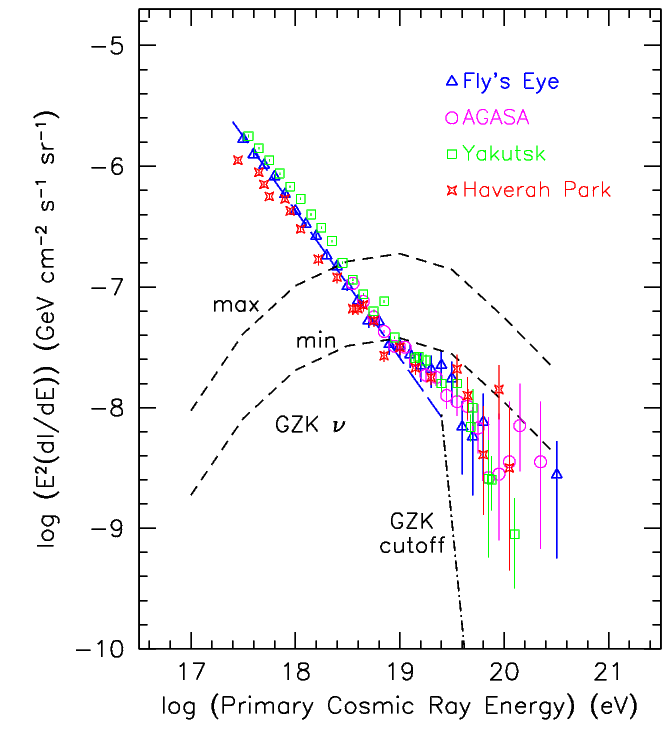
\includegraphics[width=3.25in]{crfluxes.png}}
\caption{\it \small{Cosmic ray fluxes at the highest energies. \label{fig1}}}
  \end{center}
\end{figure}

If a full-blown numbered equation is needed, for example a Fourier transform,
you would write:

\begin{equation}
\label{FT}
\tilde{F}(\omega) = {1 \over \sqrt{2 \pi} } \int_{-\infty}^{\infty} f(t) e^{-i \omega t} dt
\end{equation}

where $\omega$ is the radian frequency, $f(t)$ is the function in the time domain,
and $\tilde{F}(\omega)$ is its complex Fourier transform partner in the frequency domain.
We describe all of the terms since, as with any equation, we need to define these if
they have not been introduced before.


\section{Results and Analysis}


Here are some of the results of the analysis. Figure~\ref{fig1}
shows a plot of something vs. something, indicating the results that
we consider to be most important in this analysis. Of course in a 
real paper we would discuss in detail the features of this plot,
but this is just a template.

You should also note that there are some special characters in latex,
that you cannot use without modification. The \$ must be preceded by the
backslash character, as must the \& and the \% characters, or they will
mess up your compiling. If you are so foolish as to need the backslash
character itself in your text....well I won't even go there.

\section{Discussion}

This optional section is used to amplify some of the analysis 
of our results, and make inferences about what it might mean to the
physics problems we are trying to address. This is a good place
to compare our results to previous work, and maybe even synthesize
some of our ideas about the work into general observations or
conclusions, which are going to be restated in brief in the next and
final section.


\section{Conclusions}

We conclude various important things, which we summarize in this section. Although we
have probably stated all of them before this, we want to reinforce how we
succeeded at reaching the goals of our paper, and what it all means for
physics. Note that some people who are scanning your paper may jump to
the conclusions to see if there is something that warrants their reading the
paper in detail, so you should be sure to include salient stuff here.

% By using \section*{} the asterisk prevents Latex from enumerating this section,
% so, for example, it does not appear in a table of contents if we made one.
\section*{Acknowledgements}
We thank our mothers and fathers for having put up with us, and our
esteemed professor for giving us more breaks than we deserved.

% the following \setlength is to force the bibliography to have no
% paragraph indentations.Can use vairous units--cm are used here.
\setlength{\parindent}{0cm}

\begin{thebibliography}{99}  % the trailing 99 controls some obscure format--just use

\bibitem{Greisen_66} K. Greisen, "End to the Cosmic Ray Spectrum?,"
{\em Phys. Rev Lett. }\textbf{ 16},748 (1966).     % {\em } for emphasis, \textbf{ } for boldface

\bibitem{Zatsepin_66} G.T. Zatsepin and V. A. Kuz'min, {\em JETP
Letters} \textbf{ 4}, 78 (1966).

\bibitem{Mannheim_01}  K. Mannheim, R.J. Protheroe, J.P. Rachen
{\sl Phys. Rev. D}\textbf{ 63} (2001) 023003.

\bibitem{AGASA_01} see AGASA contributions to 27th ICRC, Hamburg 2001 (in
press 2001);  M. Takeda, {\it et. al.}, {\sl Phys. Rev. Lett.} 
\textbf{ 81}, 1163
(1998);  N. Hayashida, {\it et. al.}, {\sl Astropart.Phys.} \textbf{ 10}, 303
(1999); N. Hayashida, {\it et. al.}, {\sl Astrophys. J.} \textbf{ 522} 225
(1999).

\bibitem{HIRES_01} T.Abu-Zayyad, {\it at. al.}, "Measurement of the Cosmic
Ray Energy Spectrum and Composition from $10^{17}$ to $10^{18.3}$ eV Using a
Hybrid Fluorescence Technique", {\sl Astrophys. J.} \textbf{ 557}, 686
(2001).

\bibitem{Sigl_99} G. Sigl, S. Lee, P. Bjhattacherjee, and S. Yoshida, {\em
Phys. Rev. D}\textbf{ 59},43504 (1999).

\bibitem{Stanev_95}  N. Hayashida et al., "Possible Clustering of the 
Most Energetic Cosmic Rays
Within a limited Space Angle Observed by the Akeno Giant Air Shower Array,"
{\sl Phys. Rev. Lett.} \textbf{ 77}, 1000 (1996).

\end{thebibliography}

\end{document}

